\ctexset{
	section={
		number=\chinese{section},
		aftername={、}
	}
}

\section{论文研究目标}
论文研究目标是面向水下观测设备布放与回收过程中的远程控制需求，设计并实现一种低功耗水下声学释放器，使其具备 SFH-MFSK 声学通信功能和不依赖目标深度的快速声线测距能力；在低信噪比（SNR）、窄带干扰与折射多径等复杂水声环境下，能够长期稳定工作，可靠接收远程指令，并实现精度可接受的距离估计。

围绕上述目标，论文工作不仅包括声学释放器的软件架构、硬件总体方案以及休眠唤醒、指令解析、释放执行和应答反馈等控制流程设计，还包括通信算法与测距算法的建模仿真、参数优化和性能验证。在通信算法方面，重点研究 SFH-MFSK 信号的帧结构设计、跳频频点组织、同步检测、非相干判决和抗窄带干扰能力；在测距算法方面，围绕传播时延估计、同步时刻提取、声线折射修正和不依赖目标深度的快速距离解算方法开展仿真分析。通过算法仿真与软硬件协同设计，建立从遥控指令生成、声学信号收发、指令判决到距离估计的完整技术链路。

在工程验证层面，论文还将湖试和海试试验作为检验系统可用性的关键环节，通过外场试验数据验证声学释放器在真实水声信道中的通信可靠性、测距稳定性和释放控制闭环效果。最终形成一套兼顾低功耗、远程声学通信、快速测距与外场应用验证的声学释放器技术方案，为水下设备的可靠布放、定位辅助和回收作业提供工程支撑。

\section{开题报告中研究内容与完成情况对比}

\begin{center}
\begin{tabular}{|p{6cm}|p{8cm}|}
\hline
\textbf{开题报告中的研究内容} & \textbf{完成情况} \\
\hline
声学释放器软硬件方案设计 & 已完成声学释放器总体方案设计、功能模块划分与软硬件协同架构设计，明确了水面甲板单元与水下声学释放器之间的闭环控制流程，并完成了指令发送、信号接收、解码判决、释放执行和应答反馈等关键模块的逻辑设计。 \\
\hline
SFH-MFSK 通信体制研究 & 已完成 SFH-MFSK 通信编解码流程、跳频组织、同步检测、频点判决与多普勒补偿等关键算法的仿真与验证，并对复杂水声环境下的抗干扰性能和链路稳定性进行了分析。 \\
\hline
测距方法研究与验证 & 已完成基于传播时延的快速测距方法研究与仿真验证，围绕同步时刻提取、时延估计、声线折射修正及不依赖目标深度的距离解算开展了分析。 \\
\hline
湖试海试试验验证 & 已完成水池测试的前期试验与水声信道SFH-MFSK传播理论可行性验证，用于检验声学释放器在真实水声信道中的通信可靠性、测距稳定性和释放控制效果，为后续海试湖试提供数据与理论支持。 \\
\hline
\end{tabular}
\end{center}

\section{目前已经完成的工作和结果}

\subsection{声学释放器软硬件方案设计}

如图\ref{fig:software-system}所示，声学释放器软件系统由水面甲板单元和水下声学释放器两部分组成，并通过水声信道实现双向信息传输。水面甲板单元主要完成人机交互、遥控指令编码、回传信号接收与解码等功能；水下声学释放器则由收发合置换能器、信号接收模块、信号解码模块、指令执行模块和应答反馈模块构成。系统工作时，操作人员在人机交互界面输入遥控指令，经遥控指令编码后转换为声信号并发送至水下端；水下声学释放器接收声信号后，依次完成信号接收、解码和指令解析，并由指令执行模块控制释放机构及相关状态监测任务。指令执行完成后，应答反馈模块对执行状态进行编码，经收发合置换能器回传至水面甲板单元，水面端再完成信号接收、解码与界面显示，从而形成“指令下发、动作执行、状态反馈”的闭环控制流程。

\begin{figure}[htbp]
\centering
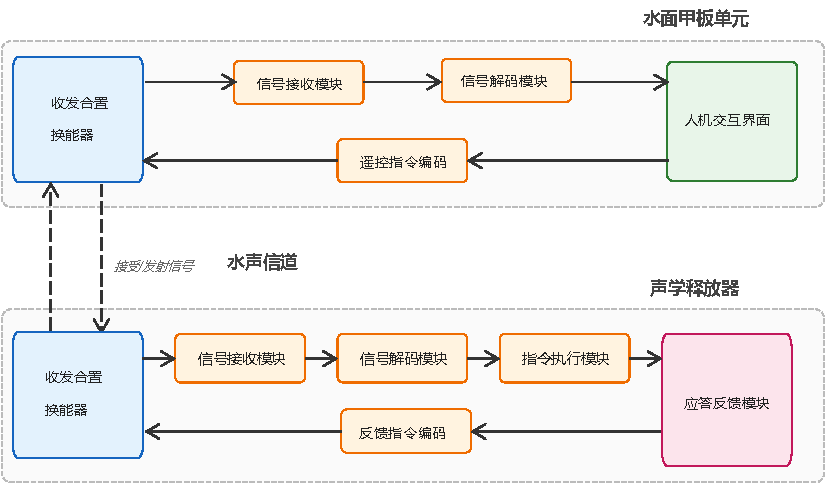
\includegraphics[width=0.95\textwidth]{software_system.pdf}
\caption{声学释放器硬件系统与工作原理示意图}
\label{fig:software-system}
\end{figure}


声学释放器的休眠唤醒与控制逻辑如图\ref{fig:sfq-logic}所示。系统启动后首先完成驱动程序配置与初始化，并进入休眠检测状态；当休眠检测电路未检测到唤醒信号时，系统保持低功耗等待状态。检测到唤醒信号后，系统开始进行信号采样，并通过两个数据缓冲区交替完成数据写入与读取，保证后续同步检测和通信解码过程能够连续进行。若同步信号在 5 min 内未到达，系统返回休眠检测流程；若检测到同步信号，则继续完成通信信号解码，并判断接收指令类型。当接收到释放指令时，系统触发声学释放器执行释放动作并完成回收；若接收到其他控制指令，则执行相应指令并发送应答信息，随后重新进入采样与判决流程。

\begin{figure}[htbp]
\centering
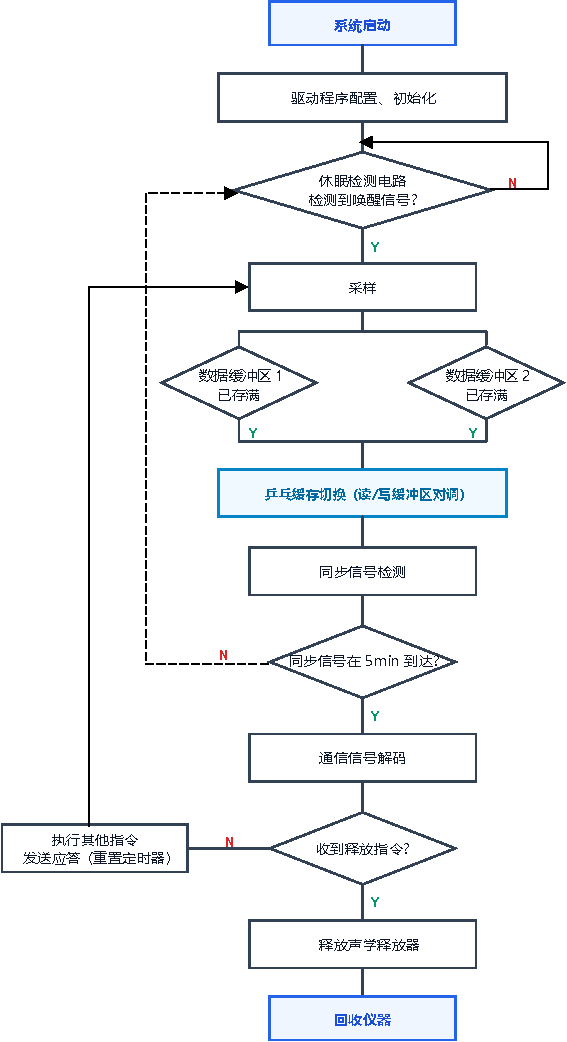
\includegraphics[width=0.72\textwidth]{sfq_logic.pdf}
\caption{声学释放器软件系统逻辑流程图}
\label{fig:sfq-logic}
\end{figure}

在通信体制设计方面，采用 SFH-MFSK 作为远程遥控指令传输与距离估计的联合信号体制。该体制通过跳频方式将信号能量分布在多个工作频点上，可降低单一窄带干扰对通信链路的影响；同时，MFSK 调制便于采用非相干检测方式实现接收判决，能够降低接收端相位同步要求，适合低功耗声学释放器的工程实现需求。结合释放器远程控制任务，帧结构设计需要同时承载控制指令信息和同步时域信息，从而为后续传播时延估计和距离解算提供基础。

围绕上述体制，已完成远程控制的总体梳理。系统处理流程可划分为指令发送端、声学接收与判决模块、释放执行单元以及测距处理模块：指令发送端负责生成控制指令并完成信号调制发送；声学接收与判决模块负责完成接收采样、同步检测、频点识别和指令判决；释放执行单元根据判决结果触发释放动作或执行其他控制任务；测距处理模块则利用同步信号和接收时刻信息进行传播时延估计，为距离计算提供输入。通过上述划分，系统的数据流和控制流已形成较清晰的闭环结构。

\subsection{FH-MFSK 信号处理流程设计与实现}

围绕 FH-MFSK 信号处理流程，已对跳频序列组织方式、频点分配原则、符号映射关系、同步检测方法以及非相干判决流程进行了分析，并据此形成了基础信号收发处理框架。在发送端，控制指令首先按照预设编码规则映射为符号序列，再结合跳频图案生成对应频点上的 MFSK 声学信号；在接收端，系统依次完成帧同步、分帧处理、能量检测、频点识别和符号判决，并将判决结果还原为控制指令。

目前已围绕接收端关键环节开展初步验证，重点检查了帧同步搜索、各候选频点能量统计、符号判决和控制指令解析之间的衔接关系。初步结果表明，现有处理框架能够支持控制信号的基本识别与解码流程，但在低信噪比、多径干扰和频偏存在时，同步检测稳定性和判决门限设置仍会直接影响通信可靠性，后续需要结合仿真和实验数据进一步优化参数。

\subsection{测距方法研究与仿真验证}

结合声学释放器应用场景，测距部分主要围绕基于传播时延的距离估计思路展开。现阶段已对影响测距误差的关键因素进行了归纳，包括同步信号检测精度、采样率设置、接收时刻判定、信道多径以及环境噪声等。由于声速剖面和声线折射会影响传播路径，后续测距模型需要在不依赖目标深度信息的条件下，对传播时间与空间距离之间的关系进行近似修正，以满足快速估计的工程需求。

基于已搭建的仿真环境，已开展若干组初步实验，对不同参数配置下的信号检测性能和距离估计趋势进行了观察。阶段性结果表明，在理想及简化信道条件下，当前收发处理流程能够实现控制信号的基本识别和处理闭环；在引入噪声与多径影响后，系统性能对同步检测方法、判决门限和参数配置较为敏感。因此，后续工作将重点围绕复杂信道下的同步鲁棒性、判决参数优化以及测距误差修正方法展开，为声学释放器的水池实验和外场应用验证提供支撑。

\section{创新点与目前取得的成果}

\subsection{创新点}

（1）针对优化算法，采用了新的算法改进措施以提升反演精度和效率。

（2）针对海试实验，采用了等效距离无关环境模型来处理距离相关的环境变化问题。

\subsection{目前取得的成果}

基于粒子滤波优化算法的地声参数反演系统 GUI 界面已开发完成。

已建立 FH-MFSK 信号收发与处理的基础框架，完成了关键算法的初步验证。

\section{后续研究计划}

\subsection{系统完善}

继续细化发送控制、接收判决、释放触发与异常处理逻辑，形成可联调的完整处理链路。

\subsection{算法优化}

重点改进 FH-MFSK 在复杂信道条件下的同步、频点判决与时延估计方法，提升通信与测距性能。

针对沉积层层数未知的地声参数反演问题，将贝叶斯优化、自回归过程模型以及分辨矩阵与粒子滤波结合，进一步提升反演精度。

\subsection{实验验证}

补充不同信噪比、传播距离和参数组合下的对照实验，定量给出识别率、误码率和测距误差等指标。
 
选取其他主流优化算法进行对比分析，明确不同优化算法在收敛速度、反演精度上的优势与局限性。

\subsection{论文写作}

同步完成实验数据整理、图表绘制和章节撰写，确保研究过程与论文形成并行推进。

\section{论文后续工作的难点与不确定性}

\subsection{主要难点}

（1）复杂水声信道带来的同步与判决难题。受时变、多径和低信噪比影响，FH-MFSK 信号在接收端的帧同步、频点识别和稳定判决存在一定不确定性。

（2）针对实际海试数据的地声参数反演问题，待反演的参数维度较高（15 个），如何在确保反演精度的前提下，显著提升计算效率和收敛速度。

（3）针对沉积层层数未知的地声参数反演问题，如何准确地确定最佳的沉积层层数，并且确保反演结果的鲁棒性和稳定性。

\subsection{不确定性}

在高维参数空间反演中，反演结果的稳定性和鲁棒性仍存在不确定性。需要进一步完善算法、增加实验验证以及改进模型选择方法。

控制通信与测距精度之间的协同优化存在不确定性，需要在有限资源下进一步权衡。

\section{指导教师意见：}
（由指导教师填写）

\vspace{24bp}
\hfill 指导教师签名：\hspace{8\ccwd}

\vspace{24bp}
\hfill 年\hspace{2\ccwd}月\hspace{2\ccwd}日
